% TITLE: Lipsum text with two figures and math
% AUTHOR: Adrian Schrader
% Created on: 31/7/15

\section{Section One}
\lipsum[1-2]

\begin{figure}[h]
  \centering
  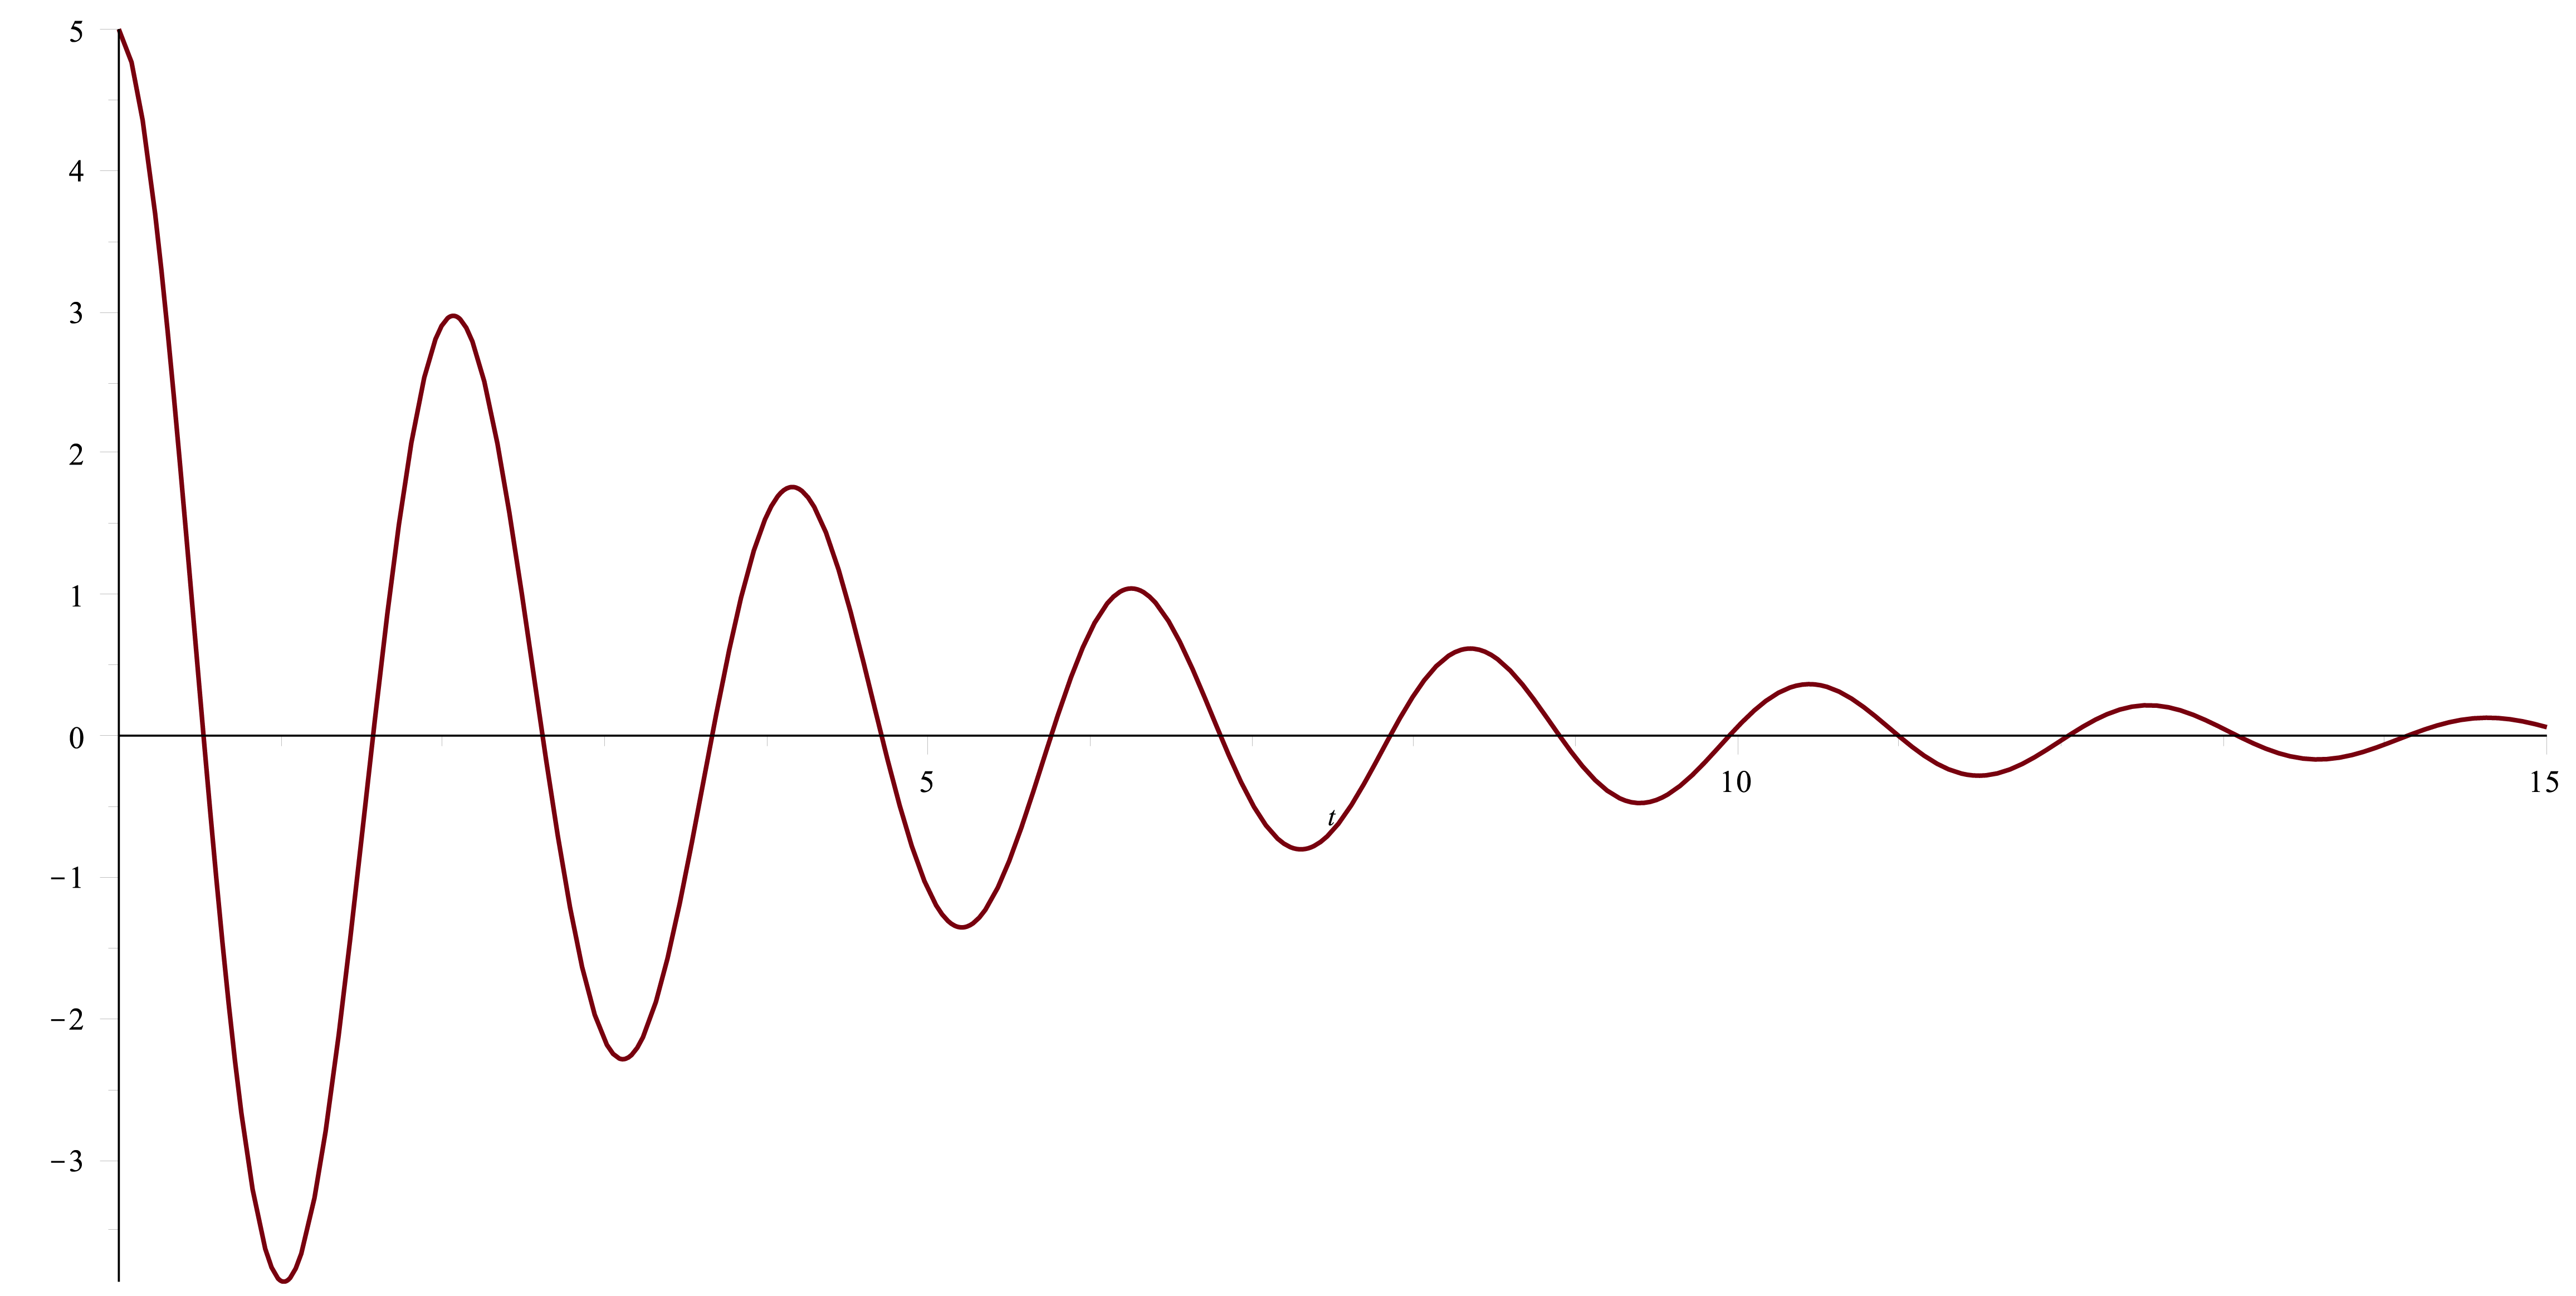
\includegraphics[width=\linewidth]{img/plot}
  \caption{Plot of of f(t) in maple}
  \label{img:function}
\end{figure}

\lipsum[3-4]

\subsection{Subsection One.One}
\lipsum[5]

\begin{figure*}[ht]
  \centering
  \includegraphics[width=\linewidth]{img/example2}
  \caption{Another Random cat picture from Google \protect\url{https://static.pexels.com/photos/4067/animal-pet-cute-cat.jpg}}
  \label{img:cat2}
\end{figure*}

\subsection{Subsection One.Two}
\lipsum[6]
\begin{figure}[h]
  \centering
  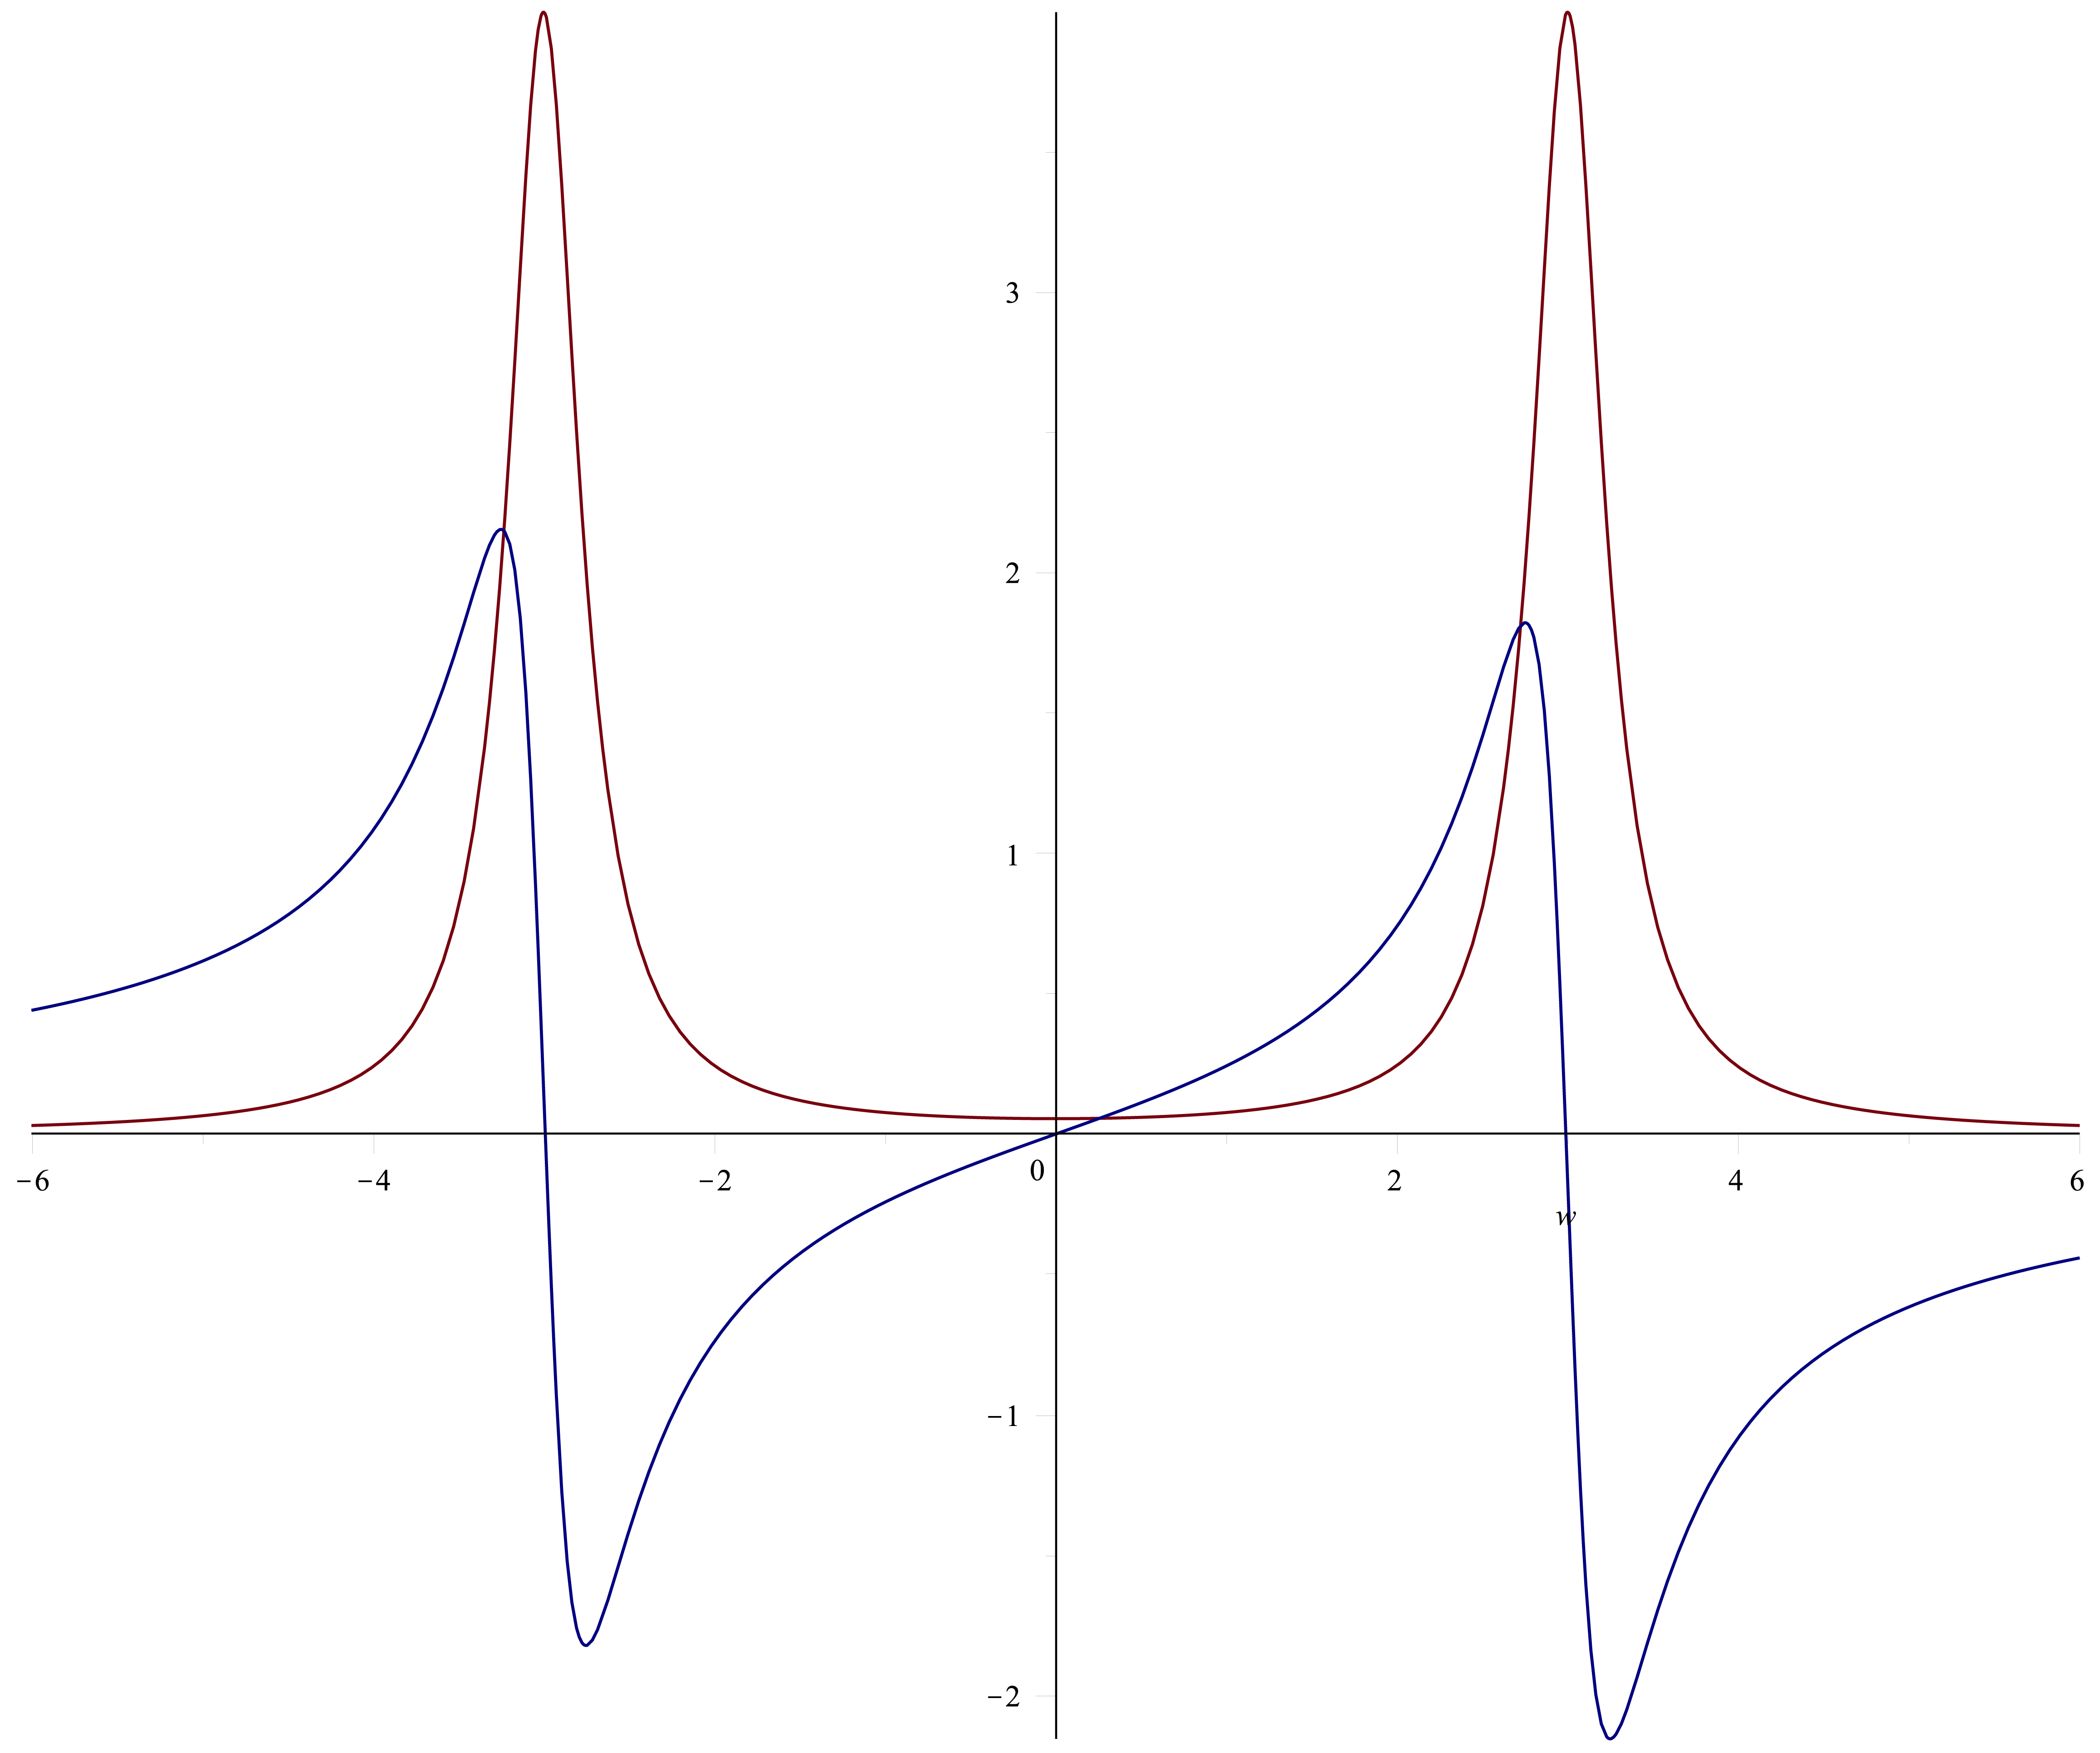
\includegraphics[width=\linewidth]{img/spectrum}
  \caption{Plot of the spectrum of f(t) in maple}
  \label{img:spectrum}
\end{figure}

\begin{align}
    f(t) &= s_0 \cdot e^{-\frac{t}{\tau}} \cdot cos(\omega_s t) \cdot \Theta(t) \nonumber \\
    &= s_0 \cdot e^{-\frac{t}{\tau}} \cdot \frac{1}{2} \Big( e^{i \omega_s t} + e^{-i \omega_s t} \Big) \cdot \Theta(t)\\
    \tilde{f}(\omega) &= \mathcal{F}(f)(\omega) = \frac{1}{\sqrt{2\pi}} \int_{-\infty}^{\infty} f(t) \cdot e^{-i \omega t} dt \nonumber\\
    &= \frac{s_0}{\sqrt{2\pi}} \frac{\frac{1}{\tau} + i \omega}{(\frac{1}{\tau} + i \omega)^2 + \omega_s^2}
\end{align}

\section{Section Two}
\lipsum[9-12]

\subsection{Subsection Two.One}
\lipsum[13-14]
